\documentclass[10pt,a4paper,final]{article}
%
\usepackage[utf8x]{inputenc}
\usepackage{ucs}
\usepackage{amsmath}
\usepackage{graphicx}
\usepackage{amsfonts}
\usepackage{amssymb}
\usepackage[spanish]{babel}
%%%%%%%%%%%%%%%%%%%%%%%%%%%%%%%%%%%%%%%%%%%%%%%%%
%%%%%%%%%%%%%%%%%%%%%%%%%%%%%%%%%%%%%%%%%%%%%%%%%
%%%%%%%%%%%%%%%%%%%%%%%%%%%%%%%%%%%%%%%%%%%%%%%%%
\begin{document}
\title{Calculo de descensos en un campo de bombeo con 2 bombas de agua}
\author{Christian N. Pfarher, Juan Pablo Garbarino, Marina Castro\\
\textit{Trabajo práctico final de ``Métodos numéricos y simulación'', II-FICH-UNL.}}
\markboth{Método numérico y simulación: TRABAJO FINAL}{}
\date{\today}
\maketitle
%%%%%%%%%%%%%%%%%%%%%%%%%%%%%%%%%%%%%%%%%%%%%%%%%
%%%%%%%%%%%%%%%%%%%%%%%%%%%%%%%%%%%%%%%%%%%%%%%%%
%%%%%%%%%%%%%%%%%%%%%%%%%%%%%%%%%%%%%%%%%%%%%%%%%
\newpage
\tableofcontents
%%%%%%%%%%%%%%%%%%%%%%%%%%%%%%%%%%%%%%%%%%%%%%%%%
%%%%%%%%%%%%%%%%%%%%%%%%%%%%%%%%%%%%%%%%%%%%%%%%%
%%%%%%%%%%%%%%%%%%%%%%%%%%%%%%%%%%%%%%%%%%%%%%%%%
\newpage
%%%%%%%%%%%%%%%%%%%%%%%%%%%%%%%%%%%%%%%%%%%%%%%%%
%%%%%%%%%%%%%%%%%%%%%%%%%%%%%%%%%%%%%%%%%%%%%%%%%
%%%%%%%%%%%%%%%%%%%%%%%%%%%%%%%%%%%%%%%%%%%%%%%%%
\section{Introducción}
medios porosos
%%%%%%%%%%%%%%%%%%%%%%%%%%%%%%%%%%%%%%%%%%%%%%%%%
%%%%%%%%%%%%%%%%%%%%%%%%%%%%%%%%%%%%%%%%%%%%%%%%%
%%%%%%%%%%%%%%%%%%%%%%%%%%%%%%%%%%%%%%%%%%%%%%%%%
\section{Objetivos}
que queremos hacer....
\begin{figure}[tbhp]
\centerline{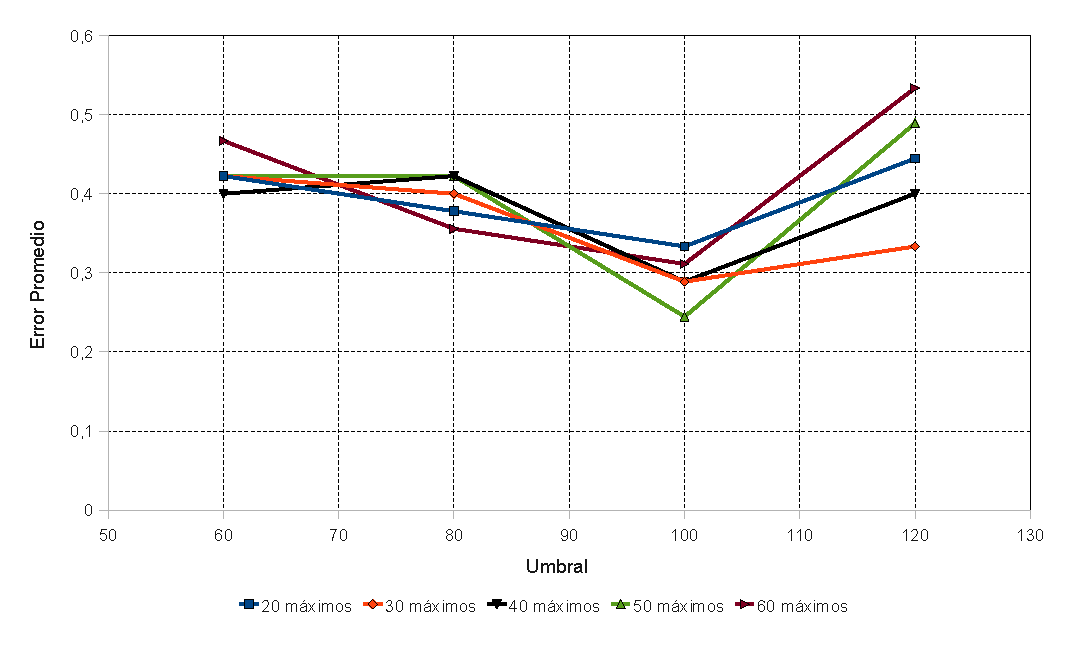
\includegraphics[scale=0.75]{img/estadistica_noche_iguales}}
\caption{Influencia de las constantes de penalización $\gamma$.}
\label{fig2}
\end{figure}
%%%%%%%%%%%%%%%%%%%%%%%%%%%%%%%%%%%%%%%%%%%%%%%%%
%%%%%%%%%%%%%%%%%%%%%%%%%%%%%%%%%%%%%%%%%%%%%%%%%
%%%%%%%%%%%%%%%%%%%%%%%%%%%%%%%%%%%%%%%%%%%%%%%%%
\section{Base Teórica}
básicamente es la ecuación de poisson con k
representado la permeabilidad.
\subsection{modelo matemático o fisico.. ver}
describir mod mate.
 son las ecuaciones matemáticas, en nuestro caso las
ecuaciones de navier stokes
%
\subsection{modelo numérico}
describir mod num.
tdyn resuelve en el espacio por el método de
elementos finitos y temporalmente hay que fijarse que opción está
tildada.
%%%%%%%%%%%%%%%%%%%%%%%%%%%%%%%%%%%%%%%%%%%%%%%%%
%%%%%%%%%%%%%%%%%%%%%%%%%%%%%%%%%%%%%%%%%%%%%%%%%
%%%%%%%%%%%%%%%%%%%%%%%%%%%%%%%%%%%%%%%%%%%%%%%%%
\section{Desarrollo}
%
\subsection{Definición de Geometría}
aca escriboC
%
\subsection{Propiedades del medio y de los materiales}
Características de Fluido: Flujo laminar, se comporta como viscoso por
la velocidad lenta.

%
\subsection{Condiciones de borde}
Condiciones de contorno: sacarlas del proyecto, enumerarlas y decir
que representa cada condición en nuestro problema. Recordar que
tenemos una condición que es la que calcula la función.
%
\subsection{Mallado}
aca escriboC
%
\subsection{Condiciones temporales}
describir como oelegimos en
%
%
\subsection{Ejecución}
cambiar el titulo esto es como se llevo a cabao la corrida
%%%%%%%%%%%%%%%%%%%%%%%%%%%%%%%%%%%%%%%%%%%%%%%%%
%%%%%%%%%%%%%%%%%%%%%%%%%%%%%%%%%%%%%%%%%%%%%%%%%
%%%%%%%%%%%%%%%%%%%%%%%%%%%%%%%%%%%%%%%%%%%%%%%%%
\section{Resultados}
v(veloc) -> lineas de flujo/vect
p->equipotenciales
realizar cortes
%%%%%%%%%%%%%%%%%%%%%%%%%%%%%%%%%%%%%%%%%%%%%%%%%
%%%%%%%%%%%%%%%%%%%%%%%%%%%%%%%%%%%%%%%%%%%%%%%%%
%%%%%%%%%%%%%%%%%%%%%%%%%%%%%%%%%%%%%%%%%%%%%%%%%
\section{Conclusiones}
si el mod respondio
que problemas tuvimos? ahi hacer mencion al pozo grande y tiempo de calculo...
pozo real vs pozo simulado
%%%%%%%%%%%%%%%%%%%%%%%%%%%%%%%%%%%%%%%%%%%%%%%%%
%%%%%%%%%%%%%%%%%%%%%%%%%%%%%%%%%%%%%%%%%%%%%%%%%
%%%%%%%%%%%%%%%%%%%%%%%%%%%%%%%%%%%%%%%%%%%%%%%%%
\end{document}